\documentclass{article}
\usepackage{amsmath}
\usepackage{tikz}
\usetikzlibrary{positioning}

\begin{document}

\textbf{Bounding Boxes with Dimension Priors and Location Prediction, adapted from~\cite{RF.17}.} The center coordinates of the box can be calculated with the predicted values \( t_\mathrm{x}, t_\mathrm{y} \) using a sigmoid function and offset by the location of grid cell \( c_\mathrm{x}, c_\mathrm{y} \). The width and height of the final box are adjusted to the previous width \( p_\mathrm{w} \) and height \( p_\mathrm{h} \) and scaled by \( e^{t_\mathrm{w}} \) and \( e^{t_\mathrm{h}} \).

\begin{figure}[h]
    \centering
    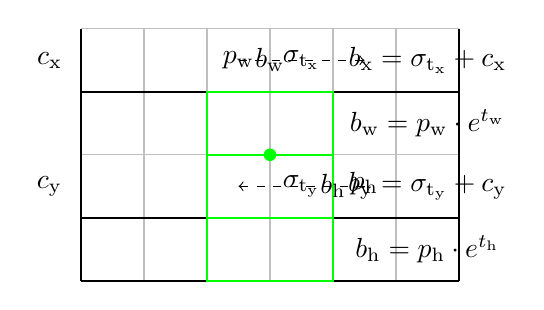
\begin{tikzpicture}[scale=0.8]
        % Grid lines
        \draw[gray!50] (0,0) grid (6,4);
        
        % Grid cell labels
        \node at (-0.5, 3.5) {$c_\mathrm{x}$};
        \node at (-0.5, 1.5) {$c_\mathrm{y}$};
        
        % Box dimensions
        \node at (2.5, 3.5) {$p_\mathrm{w}$};
        \node at (4.5, 1.5) {$p_\mathrm{h}$};
        
        % Box centers
        \fill[green] (3, 2) circle (0.1);
        
        % Box widths and heights
        \node at (5.5, 3.5) {$b_\mathrm{x} = \sigma_\mathrm{t_x} + c_\mathrm{x}$};
        \node at (5.5, 1.5) {$b_\mathrm{y} = \sigma_\mathrm{t_y} + c_\mathrm{y}$};
        \node at (5.5, 2.5) {$b_\mathrm{w} = p_\mathrm{w} \cdot e^{t_\mathrm{w}}$};
        \node at (5.5, 0.5) {$b_\mathrm{h} = p_\mathrm{h} \cdot e^{t_\mathrm{h}}$};
        
        % Sigmoid functions
        \draw[->, dashed] (2.5, 3.5) -- (4.5, 3.5);
        \draw[->, dashed] (4.5, 1.5) -- (2.5, 1.5);
        
        % Grid cell positions
        \draw[black, thick] (0, 3) -- (6, 3);
        \draw[black, thick] (0, 1) -- (6, 1);
        \draw[black, thick] (0, 0) -- (6, 0);
        \draw[black, thick] (0, 0) -- (0, 4);
        \draw[black, thick] (6, 0) -- (6, 4);
        
        % Box boundaries
        \draw[green, thick] (2, 2) rectangle (4, 3);
        \draw[green, thick] (2, 1) rectangle (4, 2);
        \draw[green, thick] (2, 0) rectangle (4, 1);
        
        % Box dimensions labels
        \node at (3.5, 3.5) {$\sigma_\mathrm{t_x}$};
        \node at (3.5, 1.5) {$\sigma_\mathrm{t_y}$};
        
        % Box centers labels
        \node at (3, 3.5) {$b_\mathrm{w}$};
        \node at (4, 1.5) {$b_\mathrm{h}$};
    \end{tikzpicture}
\end{figure}

\end{document}